\subsection*{Завдання1:}
\textbf{Рівняння Вольтера-Лотки (еволюційне рівняння) в динаміці популяцій
<хижак-жертва>:}

\begin{equation}
    \label{eq:1}
    \left\{\begin{aligned}
        \frac{dy}{dt} &= -cy + pxy \\ 
        \frac{dx}{dt} &= ax - byx
    \end{aligned}\right.
\end{equation}

\begin{figure}[h]
    \begin{minipage}[h]{0.49\linewidth}
        %% Creator: Inkscape 1.0 (4035a4f, 2020-05-01), www.inkscape.org
%% PDF/EPS/PS + LaTeX output extension by Johan Engelen, 2010
%% Accompanies image file 'pr1_1.pdf' (pdf, eps, ps)
%%
%% To include the image in your LaTeX document, write
%%   \input{<filename>.pdf_tex}
%%  instead of
%%   \includegraphics{<filename>.pdf}
%% To scale the image, write
%%   \def\svgwidth{<desired width>}
%%   \input{<filename>.pdf_tex}
%%  instead of
%%   \includegraphics[width=<desired width>]{<filename>.pdf}
%%
%% Images with a different path to the parent latex file can
%% be accessed with the `import' package (which may need to be
%% installed) using
%%   \usepackage{import}
%% in the preamble, and then including the image with
%%   \import{<path to file>}{<filename>.pdf_tex}
%% Alternatively, one can specify
%%   \graphicspath{{<path to file>/}}
%% 
%% For more information, please see info/svg-inkscape on CTAN:
%%   http://tug.ctan.org/tex-archive/info/svg-inkscape
%%
\begingroup%
  \makeatletter%
  \providecommand\color[2][]{%
    \errmessage{(Inkscape) Color is used for the text in Inkscape, but the package 'color.sty' is not loaded}%
    \renewcommand\color[2][]{}%
  }%
  \providecommand\transparent[1]{%
    \errmessage{(Inkscape) Transparency is used (non-zero) for the text in Inkscape, but the package 'transparent.sty' is not loaded}%
    \renewcommand\transparent[1]{}%
  }%
  \providecommand\rotatebox[2]{#2}%
  \newcommand*\fsize{\dimexpr\f@size pt\relax}%
  \newcommand*\lineheight[1]{\fontsize{\fsize}{#1\fsize}\selectfont}%
  \ifx\svgwidth\undefined%
    \setlength{\unitlength}{289.26128237bp}%
    \ifx\svgscale\undefined%
      \relax%
    \else%
      \setlength{\unitlength}{\unitlength * \real{\svgscale}}%
    \fi%
  \else%
    \setlength{\unitlength}{\svgwidth}%
  \fi%
  \global\let\svgwidth\undefined%
  \global\let\svgscale\undefined%
  \makeatother%
  % \resizebox*{\sz}{\sz}{%
  \begin{picture}(1,1)%
    \lineheight{1}%
    \setlength\tabcolsep{0pt}%
    \put(0,0){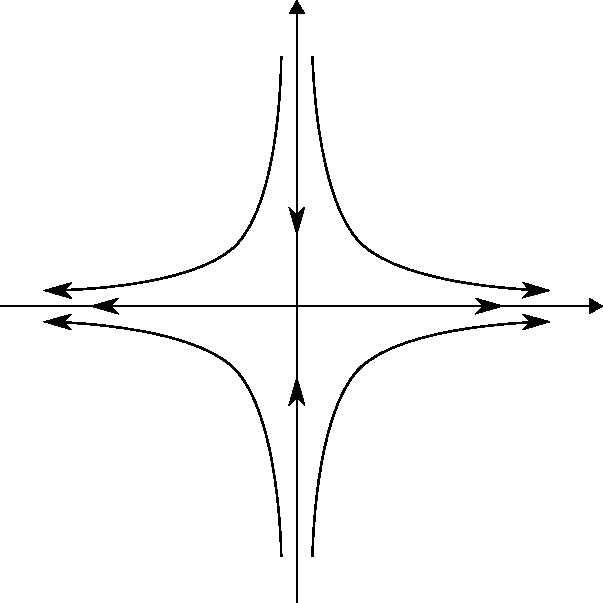
\includegraphics[width=\unitlength,page=1]{practices/1_pr/source/pr1_1.pdf}}%
    \put(0.42420684,0.92372983){\color[rgb]{0,0,0}\makebox(0,0)[lt]{\lineheight{1.25}\smash{\begin{tabular}[t]{l}$Y$\end{tabular}}}}%
    \put(0.8969896,0.43585215){\color[rgb]{0,0,0}\makebox(0,0)[lt]{\lineheight{1.25}\smash{\begin{tabular}[t]{l}$X$\end{tabular}}}}%
  \end{picture}%
  % }
\endgroup%
 \\
        \centering {a)}
    \end{minipage}
    \begin{minipage}[h]{0.49\linewidth}
        %% Creator: Inkscape 1.0 (4035a4f, 2020-05-01), www.inkscape.org
%% PDF/EPS/PS + LaTeX output extension by Johan Engelen, 2010
%% Accompanies image file 'pr1_2.pdf' (pdf, eps, ps)
%%
%% To include the image in your LaTeX document, write
%%   \input{<filename>.pdf_tex}
%%  instead of
%%   \includegraphics{<filename>.pdf}
%% To scale the image, write
%%   \def\svgwidth{<desired width>}
%%   \input{<filename>.pdf_tex}
%%  instead of
%%   \includegraphics[width=<desired width>]{<filename>.pdf}
%%
%% Images with a different path to the parent latex file can
%% be accessed with the `import' package (which may need to be
%% installed) using
%%   \usepackage{import}
%% in the preamble, and then including the image with
%%   \import{<path to file>}{<filename>.pdf_tex}
%% Alternatively, one can specify
%%   \graphicspath{{<path to file>/}}
%% 
%% For more information, please see info/svg-inkscape on CTAN:
%%   http://tug.ctan.org/tex-archive/info/svg-inkscape
%%
\begingroup%
  \makeatletter%
  \providecommand\color[2][]{%
    \errmessage{(Inkscape) Color is used for the text in Inkscape, but the package 'color.sty' is not loaded}%
    \renewcommand\color[2][]{}%
  }%
  \providecommand\transparent[1]{%
    \errmessage{(Inkscape) Transparency is used (non-zero) for the text in Inkscape, but the package 'transparent.sty' is not loaded}%
    \renewcommand\transparent[1]{}%
  }%
  \providecommand\rotatebox[2]{#2}%
  \newcommand*\fsize{\dimexpr\f@size pt\relax}%
  \newcommand*\lineheight[1]{\fontsize{\fsize}{#1\fsize}\selectfont}%
  \ifx\svgwidth\undefined%
    \setlength{\unitlength}{355.43820839bp}%
    \ifx\svgscale\undefined%
      \relax%
    \else%
      \setlength{\unitlength}{\unitlength * \real{\svgscale}}%
    \fi%
  \else%
    \setlength{\unitlength}{\svgwidth}%
  \fi%
  \global\let\svgwidth\undefined%
  \global\let\svgscale\undefined%
  \makeatother%
  % \resizebox*{\sz}{\sz}{%
  \begin{picture}(1,1)%
    \lineheight{1}%
    \setlength\tabcolsep{0pt}%
    \put(0,0){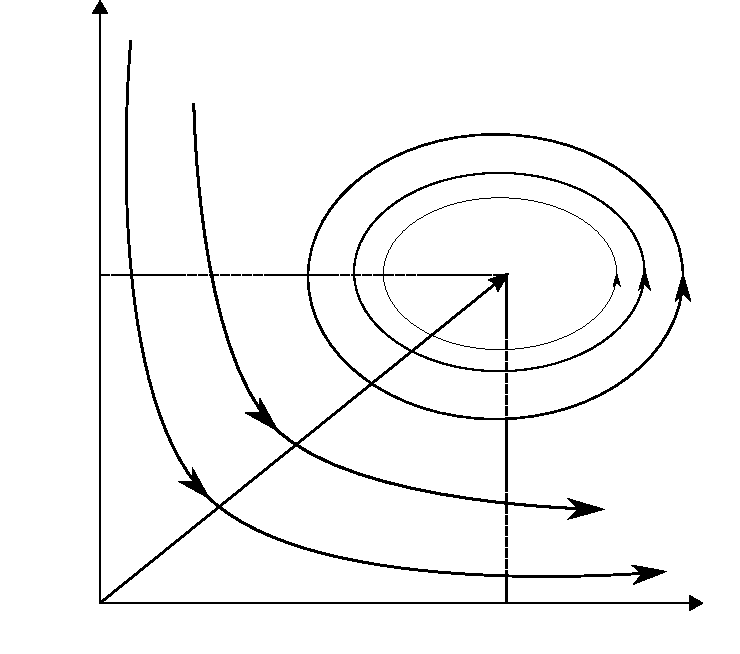
\includegraphics[width=\unitlength,page=1]{practices/1_pr/source/pr1_2.pdf}}%
    \put(0.1,0.83){\color[rgb]{0,0,0}\makebox(0,0)[lt]{\lineheight{1.25}\smash{\begin{tabular}[t]{l}$Y$\end{tabular}}}}%
    \put(0.9,0.03){\color[rgb]{0,0,0}\makebox(0,0)[lt]{\lineheight{1.25}\smash{\begin{tabular}[t]{l}$X$\end{tabular}}}}%
    \put(0.097,0.49295599){\color[rgb]{0,0,0}\makebox(0,0)[lt]{\lineheight{1.25}\smash{\begin{tabular}[t]{l}$Y_0$\end{tabular}}}}%
    \put(0.668,0.03){\color[rgb]{0,0,0}\makebox(0,0)[lt]{\lineheight{1.25}\smash{\begin{tabular}[t]{l}$X_0$\end{tabular}}}}%
    \put(0.3,0.25){\color[rgb]{0,0,0}\makebox(0,0)[lt]{\lineheight{1.25}\smash{\begin{tabular}[t]{l}$\overrightarrow{u}_0$\end{tabular}}}}%
  \end{picture}%
  % }
\endgroup%
 \\
        \centering{b)}
    \end{minipage}
\end{figure}



\textbf{знайти особливі точки (M(0,0), N($\frac{c}{p},\frac{a}{b}$))}

Потрібно прирівняти рівняння (\ref{eq:1}) до нуля і розв'язати:
$
    \left\{\begin{aligned}
        -cy + pxy = 0\\
        ax - byx = 0
    \end{aligned}\right.
$

\begin{enumerate}
    \item {
        Припустимо, що $x=0$, тоді $y=0$
    }
    \item {
        Припустимо, що $x \ne 0$, тоді з другого рівняння випливає:
        $$ x(a-by) = 0 \Longrightarrow a-by = 0 \Longrightarrow y = \frac{a}{b}$$
        відповідно :
        $$ -c\frac{a}{b} + px\frac{a}{b} \Longrightarrow x = \frac{c}{p}$$
    }
\end{enumerate}

\textbf{написати рівняння фазових траєкторій}

$\frac{dy}{dx} = \frac{y(-c+px)}{x(a-by)} \ \ \cdot \frac{\frac{1}{xy}}{\frac{1}{xy}}$ 

$\frac{dy}{dx} = \frac{\frac{-c + px}{x}}{\frac{a-by}{y}}$

$dy\frac{a-by}{y} = dx\frac{-c + px}{x}$

$a\ln y - by = -c\ln x + px + C\ \ | b=p =1$ 

$x + y -c\ln x -a\ln y = C$ : Інтеграл руху (еволюції)


\textbf{Довести тотожність:}

$x + y -c\ln x -a\ln y = C$

$\frac{d}{dt}(x + y -c\ln x -a\ln y) = \frac{d}{dt}C$ 

$ax - yx - cy + xy -\frac{c}{x}(ax-yx)  - \frac{a}{y}(-cy +xy) = 0$

$\textcolor{red}{ax} \textcolor{blue}{- xy} - cy \textcolor{blue}{+ xy} \textcolor{green}{-ac} + cy \textcolor{green}{+ ac} \textcolor{red}{- ax} = 0$


\textbf{Знайти $\dive \overrightarrow{v}$}

$\dive \overrightarrow{v} = \frac{\partial v_1 }{\partial x} + \frac{\partial v_2}{\partial y } = 
a - by - c +px = a - c -by + px$



\textbf{Знайти $\Gamma $}

$\ln \Gamma = (a - c - by + px) t + C$

$\Gamma(t) = \Gamma(0)e^{(a- c - by +px)t}$